\documentclass[11pt]{article}
\usepackage[usenames, dvipsnames]{color}
\definecolor{pass_grn}{RGB}{0, 230, 0}
\definecolor{fail_red}{RGB}{230, 0, 0}
\usepackage{fancyhdr}
\usepackage{adjustbox}
\usepackage[a4paper, total={6in, 8in}]{geometry}
\usepackage{graphicx}
\usepackage{listings}
\usepackage{multirow}
\usepackage{pifont}
\newcommand{\cmark}{\ding{51}}%
\newcommand{\xmark}{\ding{55}}
\usepackage{subcaption}
\usepackage{titling}
\usepackage[nottoc,numbib]{tocbibind}
\usepackage{wrapfig}
\pagestyle{fancy}
\fancyhead{}
\renewcommand{\headrulewidth}{0pt}
\fancyfoot[LE,RO]{Y1481702}
\newcommand{\myparagraph}[1]{\paragraph{#1}\mbox{}\\}

\title{Software Testing}
\author{Y1481702}
\date{\today}
\setlength\parindent{0pt}

%\setlength{\droptitle}{-2em} %ADJUST HEIGHT OF TITLE
%\addtocontents{toc}{\protect\setcounter{tocdepth}{2}} %ADJUST WHICH SECTIONS APPEAR IN CONTENTS TABLE

\begin{document}
\begin{titlepage}
\clearpage\maketitle
\thispagestyle{empty}
\tableofcontents
\end{titlepage}

%Your report must not exceed 10 sides of A4, minimum of 11pt font
%minimum 120% line spacing
%o: correct, see https://tex.stackexchange.com/questions/348678/how-to-set-document-line-spacing-in-pt-format
%minimum 2cm margins on all sides

%does not include covering page, table of contents or reference list

%EXAM NUMBER SHOULD BE WRITTEN ON THE FRONT PAGE AND ALL SUBSEQUENT PAGES
%APPROX ONE PAGE PER 10 MARKS:


%GENERAL ADVICE:
	%You won’t receive marks for testing that the marker merely thinks you probably did — marks will only be awarded for tests that are described explicitly and precisely.
	%Yes, it is a little unrealistic that you are only allowed 10 pages and 8 tests, and that your possible coverage and comprehensiveness are limited by that. However, in the real world there are always resource limits — the ones you have here are merely artificial ones.
	%Do not repeat anything that does not vary. For example, do not repeat the same boilerplate text in every test case description — if something is true for all test cases, say this once at the start of the section.
	%Similarly, use blanket statements to make points that are true of multiple (but not all) tests case (e.g. “Test cases 1–5 assume that...”)
	%Appendices containing full JUnit code or detailed test output etc are not required and will not be read.
	%In general, do not waste space on spurious information. Think about what the notional target reader needs to know in order to use your document, and include only that. At best, other information will waste some of the limited pages available to you.
	%If you reference an external document (such as the documentation or website for the software you are testing), be sure to cite it appropriately, just as in any other submitted work.

\section{Test Plan}% 25 Marks (2.5 pages)
%A test plan
%It should detain the methods used to build the test cases and the software tools used to achieve these
\subsection{Introduction}
%o: What is JAVA MASON?
MASON is a software library for creating agent-based simulations in Java. 
%o: From a testing point of view MASON is a form of OPEN SOURCE SHRINKWRAP
	%may be used in the wild by many people
	%what other ramifications does this have
The software fits into the category of shrinkwrap meaning it might be in use in a wide range of real-world production environments. The software is freely-available and open-source, which is a special case of shrinkwrap software. A common trait of open-source software is that tasks 'that are not considered "fun" often don't get done'.\cite{five_worlds}
%As open source software is often developed without anyone being paid,
	%only "fun" things are done
	%i.e. NOT TESTING
For MASON in particular, it is likely that the software has not been thoroughly tested as there is no trace of any automated testing, either on the MASON website, or its GitHub repository.
This report documents testing of the latest version (19.0) of MASON, which has been obtained from the MASON website, with the aim to discover whether this software is dependable.
%usage statistics can provide with an estimate of how well it needs to work
%biological simulations- high profile studies have based hypotheses on this framework

\subsubsection{Tools}
The IntelliJ IDE was used to explore the code and develop automated tests.
This IDE gives powerful features, including plugins for generating code metrics and displaying coverage of unit testing.
Specifically, the MetricsReloaded plugin\cite{metrics_reloaded} has been used for generating the statistics in Fig. \ref{tables:metrics}.
\\

JUnit has been used to create automated testing for the software, this includes both unit and integration testing.
Git version control has been used to manage the code for these JUnit tests.
For a long term project, this would be particularly advantageous as any automated tests could be updated and versioned alongside any future code changes.

\subsection{Test Coverage}
\subsubsection{System Overview}
%Explain the overall strategy you used for creating test cases, and for selecting the specific test cases that you present in section B
In order to design appropriate test cases an understanding of all levels of the system was needed. As resources here are significantly limited, with only 8 testcases are allowed, it will be necessary to ensure they are used in the most effective way.
%Clearly define what constitutes "the software under test" and list the features that you will test and not test
As stated in the project brief, the testing only needs to cover the following packages, but not their subpackages:

\begin{itemize}
\item \texttt{sim.engine} is responsible for the core simulation management, including the agent scheduling.
\item \texttt{sim.field} provides abstract classes for the representations of space in MASON simulation models, with subpackages managing specific instances of these.
\item \texttt{sim.field.grid} provides various 2D and 3D grid representations of simulation space.
\end{itemize}

Fig. \ref{fig:loc} shows the proportional sizes of each of these three modules, while Fig. \ref{fig:uml} shows their code components. 
\\

It has been shown across software projects that some modules of code may be significantly more error prone than others.
The Pareto principle is said to hold with software bugs, with 80\% of software bugs being found within 20\% of the code\cite[pp. 124]{pressman}.
We can use a variety of metrics about our software to predict which parts of the code that these bugs may be hiding in\cite{predicting_from_history}.
Unfortunately, a number of these metrics, including a history of bugs are not publicly available.
\\

%Complexity:
High cyclomatic complexity (Fig. \ref{fig:cc}/Fig. \ref{table:cc}) can be a good indicator of the most bug-ridden sections of applications.
The causality here can be easily understood: complexity creates confusion which results in developers misunderstanding the software they are trying to build.
This misunderstanding can provoke a large number of bugs in the code.
The graphs show that \texttt{sim.field.grid} has a slightly higher share of the code's complexity than lines of code.
%FIND GRAPH THAT SHOWS DISPROPORTIONATE COMPLEXITY BETWEEN sim.field.grid classes!
If we investigate this metric in further detail, it becomes clear that the majority of the more complex classes are in the \texttt{sim.field.grid} package.
This metric has been plotted against the number of changes that have been committed to the class' source file.
Files which are subject to frequent change have had more opportunity to develop additional bugs, therefore files with high complexity and frequent changes are particularly worrying and should be looked at.
\\

%Dependency:
Fig. \ref{table:dependency} shows how the packages in the test scope interact with other packages in the system.
In particular, \texttt{sim.engine} is directly relied upon by a large number of other packages.
%Code Coverage during simulation/runtime?
Additionally, code coverage (Fig. \ref{fig:coverage_heatbugs}) has provided a good understanding of which parts of the software are regularly used while running simulations.
Again \texttt{sim.engine} appears to be heavily used by the demo simulations.
\\

\begin{figure}
\begin{subfigure}[b]{0.5\textwidth}
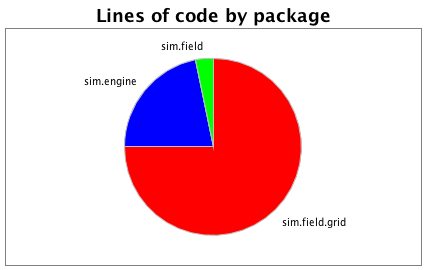
\includegraphics[width=\textwidth]{Appendix/LOC}
\caption{Lines of Code}
\label{fig:loc}
\end{subfigure}
\begin{subfigure}[b]{0.5\textwidth}
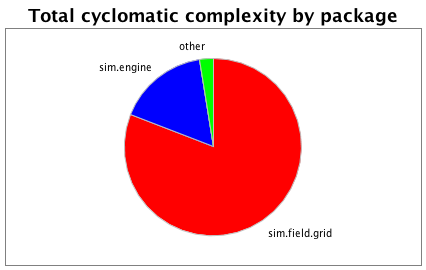
\includegraphics[width=\textwidth]{Appendix/Cyclomatic}
\caption{Cyclomatic Complexity}
\label{fig:cc}
\end{subfigure}

\caption{Charts showing various metrics of MASON}
\label{fig:metric_charts}
\end{figure}

%much of the project is several years old.. why is this?
%	stable to not require updating

%are there any special features of the packages that are notable for testing?
%	UI Testing is hard to test - See Lecture 6
%	OO Code is hard to test
%	concurrency	

%how do we know how a general user works?
%examples of real-world usage (PPSim), vs mason tutorials


\subsubsection{Testing Goals}
%Define acceptability criteria for the software - what (testable) properties does it need to have in order for it to be acceptable quality for its intended purpose?
%o: These will help define the goals of our testing:
	%find the maximum number of bugs?
	%know whether we have undiscovered bugs?
	%o: ^^THIS IS THE MAIN GOAL HERE- 'the institute would like to know if they can really trust the system to be dependable'
	%'want you to provide a thorough assessent of its freedom from defects'
	%comply with regulator-set demands

	%have a compelling defence in a courtcase (self-driving cars, too soon?)
	%minimum time and cost?
		%obviously here we have a set TIME- open assessment for 10 credit module
There are a number of goals we could define for our testing, such as finding the maximum number of bugs or complying with regulator set demands.
The given requirement here is to verify, with a limited number of resources, that the software is dependable.
In general, it's better to test with the aim of showing a product fails, if we cannot do so then the product is reliable enough\cite[pp. 20]{lessons_book}.
As such, the main requirement for our testing is to find any significant undiscovered bugs in commonly used code.
\\
%In many projects, most requirements come from inference or implicit specifications
%if a product violates an explicit spec: "it violates the spec, it is wrong"
%if a product violates an implicit spec, you have to make a case: "it does this.. which is unexpected, this may confuse users, who do x in their daily work."

%"IT WORKS" means it appears to meet some requirement.. to some degree
%--ALL FROM \cite{lessons_book}

Due to limited resources, the tests will aim to cover the parts of the software which are likely to be used more often by the target users.
In this case, our target users are the staff of a private biological research institute.
The brief has not provided any specific use cases for the software, so this aim will not be trivial to accomplish.
Previous biological implementations which utilised MASON\cite{ppsim} have been used to gain an insight into which MASON features are important to biological simulations.
\\

Additionally I have assumed that MASON's bundled demo simulations give typical use cases for the library.
Running these simulations with code coverage detection turned on has given a good overview of which parts of the code are used regularly (Fig. \ref{fig:coverage_heatbugs}).
Core simulation code that is used routinely by all simulations regardless of their customisations should be tested the most rigourously.
Both the documentation\cite[pp.85]{mason_doc} and code coverage checks indicate that this type of code can be found within \texttt{sim.engine}.

%TODO: THE SYSTEM WILL BE ACCEPTABLE : IF

\subsubsection{Expected Behaviour}
%usage by a private biological research institute
%users will be research scientists with BASIC Java training
%Explain how you have determined the expected behaviour of the software (in the absense of an exhaustive and explicit requirements specification)
The expected behaviour of the software has been determined using the extensive MASON documentation\cite{mason_doc} and first-party example implementations.
Many of these examples have been implemented using the ContinuousGrid classes which are outside of the test scope.

The MASON documentation has conflicts, likely caused by parts of the document becoming out of date as the software is updated.
One example of this is that in the tutorial section on Page 19, it describes different behaviour for the \texttt{-time} command line argument to that described in the formal documentation on page 91.
In this case, and in general, the behaviour in the main documentation has been assumed correct and the tutorials assumed to be out of date.
If a more ambiguous case had presented itself, exploratory testing could have been used to determine the expected behaviour.

%what IS this expected behaviour: we are able to create and run agent-based simulations?

\subsubsection{Unit Testing}
Unit Testing allows the testing of small sections of source code.
In this case, unit tests will help us to isolate the select packages that are within the scope of testing from the rest of the system.
\\

Unit testing should focus on core code that is a dependency for other modules, code that regularly gathers bugs and code that is changed by a number of different developers.
It should not cover trivial code, such as accessors and mutators, code with non-deterministic results or UI code.\cite{dont_test_blindly}
In this case, we will target our unit testing at ensuring the core software functionality is correct, specifically that simulations can be created and run.
%Unit Test: sim.engine?
		   %sim.field.. whichever grid is most relevant to biologists?
\\

As previously mentioned, it has been shown that approximately 20\% of the code, contains 80\% of our program's bugs.
Our unit testing will aim for 60-70\% code coverage of core code and \textasciitilde 20\% of the overall application, as recommended in \cite{dont_test_blindly}.

\subsubsection{Integration Testing}
%testing interacting classes..
	%focus on communication and flow of information between the modules

Java is a heavily object-oriented (OO) language. This will affect our testing as in this type of software, much of the complexity is moved from algorithms in methods, to the connection of software components\cite[pp.236]{introduction_book}. We will therefore need a much greater focus on integration testing than unit testing.

%not fully within the scope of our testing, we have only been asked to test
	%sim.engine
	%sim.field
	%sim.field.grid

	%we can test the way these packages interact...
	%classes within these packages interact?

%three main approaches to this:
	%big bang
	%top down
	%bottom-up

\subsubsection{System Testing}
%In this case 'the system is our selected packages'
While testing the system as a whole will not help us find low-level bugs, it will give a high-level view of whether the bulk of the functionality appears to work as expected.
System testing of the application will be conducted using the MASON UI as a black-box test. As such, although the test relies on functionality provided by classes outside the test scope, the test cases will only attempt to verify functionality provided by classes which are in scope.
%what functional requirements are under test:
\\

System testing will also help us to verify the non-functional requirements that have been previously determined.
In particular, our system testing will cover
%non-functional requirements:
	%basic Java programming?
	%portability
	%open source

\paragraph{Acceptance Testing}
is a particularly useful form of system testing, which can be used for verifying non-functional requirements.
It can be useful for understanding the domain of our software better, but as we are not intending to further develop MASON, this is not particularly relevant here.
%HELPS ENSURE THE CUSTOMER TRUSTS OUR QUALITY CLAIM
However, it would helpful to discover if it is appropriate for the target audience.
A particularly important non-functional requirement of our software is that it can be operated effectively by our end users.
In particular, our users have supposedly only received a basic level of Java training.
It has been stated that MASON is less-suited to beginner programmers, when compared to other tools, such as NetLogo\cite{abm_platforms_review}.
\\

In order for acceptance testing to be meaningful, it should be performed on potential users.
Unfortunately, this means that this type of testing is out of reach for this report as target users are unavailable.

\subsubsection{Mutation Testing}
Mutation testing is often used to determine the effectiveness of a test-set at discovering bugs in the system.
As we already have a very limited number of tests, mutation testing will not be used.

\subsubsection{Regression Testing}
Unfortunately neither the website nor the GitHub repository for MASON provide any previously implemented automated testing.
Either this testing has not been done, which is common with freely-distributed software, or it has not been publicly distributed.
As such, it will not be possible to run any regression testing as part of the project.

\section{Test Case Specifications}% 30 Marks (3 pages)
%Test case specifications for 8 fully specified test cases. The test cases must be complementary: they must make different assumptions and test different specific features of the library.
	%At minimum, each test case should describe the stimulus applied to the software (which might be a sequence of API calls, a sequence of user actions that are taken, or something else) and the expected
		%i.e. correct behaviour
		%N.B. for some tests it may be appropriate to define constraints (e.g. "no files will be changed") instead of/as well as positive statements of behaviour (e.g. "the user will be returned to the main menu screen").
		%Where the reason why the expected/correct behaviour is indeed expected and correct is not obvious to a capable programmer where some domain knowledge, explain briefly why it is so
	%Each test case should also state the purpose of the test within the test set. A good way to do this may be to state the question that the test case asks about the software. If we cannot understand what the purpose of a given test case is, we cannot give you much credit for it.
	%“One test case” should test one thing – one feature, one unusual input, or one user task. For example, if you have a function that takes an integer as an input, testing it with Min/Max/+1/0/-1 should be five test cases. One can note that those are, however, five very low-level (unit test) test cases, which are unlikely to give you the most testing power in a fixed number of tests, and hence unlikely to give you maximum marks.
	%You should aim to provide a diverse range of test cases, and also to provide your best test cases (including any that find interesting bugs). There is an inevitable tension between these two objectives, which you will have to decide how to resolve.
	%For full marks in this section, tests should be conducted at a range of testing levels, including unit, integration and system level. Hint: explicitly label each of your tests with what level it’s working at.
	%You may include short fragments of code within your test case specifications, but not larger ones. In particular, do not include whole JUnit tests. In essence, you need to provide enough information for a smart programmer to recreate your test code given some effort. e.g. if a test case involves a specific sequences of method calls, that sequence of method calls needs to be clear from the test case description.


%o: "Black box testing means that knowledge of the internals of the product doesn't play a significant part in your testing."\cite{lessons_book}
%o: "To do black box testing well, learn about the user, their expectations and needs, the technology and configurations the software will run on, the other software that this software will interact with, the date the software must manage, the development process, and so on. The advantage of black box testing is that you probably think differently than the programmer, and, thus are likely to anticipate risks that the programmer missed."
\subsection{Test Case 1}
%Having a good understanding of the classes' intentions should ensure that the tests are also meaningful


The \texttt{AbstractGrid} classes are among those with the highest cyclomatic complexity.
The other grid classes inherit code from these abstract classes, except SparseGrid2D which duplicates a great deal of code instead (Fig. \ref{fig:dupe_code}), implying this code is highly important.
\texttt{AbstractGrid2D} also has the highest number of historic code changes out of the \texttt{sim.field.grid} package.
These two metrics are worrying given that the simulation runs show that this class is routinely used to some extent.
Unit Test cases have been derived to target the methods in this class with the highest complexity (Fig. \ref{fig:method_complexity}), specifically \texttt{getHexagonalLocations}.
\\

\texttt{AbstractGrid2D} cannot be directly instantiated for this test, so \texttt{DoubleGrid2D} will be used as it extends the class without overriding \texttt{getHexagonalLocations}.
A new \texttt{DoubleGrid2D} object is instantiated with width and height both equal to 150.
The method is called with the origin x and y both equal to 120 and dist equal to 20.
The grid mode is set to bounded, origin is set to be included and empty \texttt{IntBag}s are passed to the method.
The expected output has been independently calculated using a hexagon point algorithm.
These independently calculated point values have been manually verified as correct using a 2D graphing software.

\subsection{Test Case 2}
%no specific detail given in brief
%but previous published biological simulations using MASON have been implemented using ObjectGrid2D.
Another method of \texttt{AbstractGrid2D} which has a high cyclomatic complexity is \texttt{getRadialLocations}.
This method will also be tested to ensure its behaviour is expected.
In particular testing at boundaries is most likely to show ambiguities in the specifications\cite[pp.25]{lessons_book}, thus revealing bugs.
In the case of this method, a boundary case is checking that the values correctly wrap around when the grid is in toroidal mode.
A new \texttt{DoubleGrid2D} is created with width 200 and height 160.
The \texttt{getRadialLocations} method is invoked with an origin of (150, 150) and a radius of 20 so that the circle should wrap around the end of the grid in the y-direction.
In this case, include origin is set to true and empty \texttt{IntBag}s are passed into the method.
\\

Assertions are made to ensure that the size of the bags for x and y are both equal to 1345.
The bags are then compared against the expected values as calculated independently by the midpoint circle algorithm.
These independently calculated point values have been manually verified as correct using a 2D graphing software.
In order to check that the toroidal wrapping works correctly, the remainder operator is applied to these circle algorithm results with the height/width of the field.

\subsection{Test Cases 3-4}
\begin{wrapfigure}[22]{r}{0.4\textwidth} 
	\vspace{-25pt}
	\begin{center}
		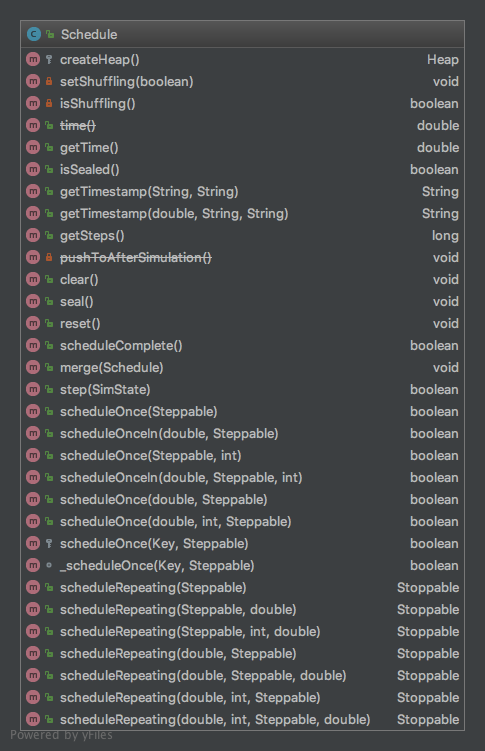
\includegraphics[width=0.4\textwidth]{Appendix/Schedule}
		\caption{Schedule Class}
		\label{fig:schedule}
	\end{center}
\end{wrapfigure}

As previously stated, our initial integration testing will focus on the simulation scheduler which provides the core functionality for MASON.
This scheduler works with the \texttt{SimState} class and custom implementations of the \texttt{Steppable} interface to provide the functionality that simulates the passing of time.
\\

While this integration between classes may appear to be complex at first glance, with numerous methods available (Fig. \ref{fig:schedule}), many of its methods are simply overloads,  due to Java's lack of real support for default function arguments.
Testing a single example of \texttt{scheduleOnce} function, will provide a reasonable assurance that the functionality works, as code is shared with each overloaded instance calling the private \texttt{\_scheduleOnce} method.
\\

\textbf{Test Case 3} will add a \texttt{Steppable} object to the \texttt{Schedule} and ensure that the \texttt{step} method work as expected.
A by-product of this test, is the assurance that the \texttt{\_scheduleOnce} method also works as expected.
As \texttt{\_scheduleOnce} is a private method, it will be called indirectly by one of its overloading methods: \texttt{scheduleOnce(Steppable)}.
Other overloading methods could be used instead with no difference on the test case as the scheduler skips any empty timesteps.
In order to facilitate this test, a simple \texttt{Increment} class (Fig. \ref{code:increment}) has been created.
The scheduler will be stepped a number of times (10) to ensure that the \texttt{Increment} value is correctly stepped.
\\

\textbf{Test Case 4} is similar, but will utilise the \texttt{scheduleRepeating(Steppable)} to ensure that the Schedule correctly manages recurring events.
As mentioned, the scheduler skips any empty timesteps, so providing a different start time or time interval will make little difference to the test.
Again, the scheduler will be stepped a number of times (10) to ensure that the value is stepped multiple times as expected.

\subsection{Test Case 5}
%Test ERROR MESSAGES: this code tends to be weaker than mainstream functionality- will be important to guide less-confident users (beginner Java)
	%:all from \cite{lessons_book}

\subsection{Test Case 6}
\subsection{Test Case 7}
This test case will verify that the tool is able to run from the command-line, correctly reacting to user configurations.
The example simulation will be run for a specified number of 
\\
The documentation here is conflicting. On Page 91, the \texttt{-time} argument specifies that it will `print a timestamp every T simulation steps' whereas page 19 states that the argument means the simulation will `run for a limited time', behaviour that 19 attributes to the \texttt{-until} argument.

\subsection{Test Case 8}
%Testing non-deterministic events is hard:
%We can perform some statistical analysis to ensure the output is expected?
This test case will verify that the tool works as expected from the User Interface.

\newpage
\section{Test Results}% 15 marks (1.5 pages)
%The test results for each of the tests that were specified in item B.
	%Here, you should document the results that occurred when the test cases are run. You should provide explicit indication of whether each test passed or failed, and in the latter case state what happened instead.

%o: screenshots may be useful, but add them in appendix?
\begin{adjustbox}{center}
\begin{tabular}{|c|c|c|p{10em}|p{10em}|p{10em}|}
	\hline
	\textbf{Case} & \textbf{Pass} & \textbf{Level} & \textbf{Expected} & \textbf{Actual} & \multicolumn{1}{c|}{\textbf{Details}} \\
	\hline
	1 & \textcolor{pass_grn}{\cmark} & Unit & A hexagonal set of points is created, such that the points match the expected values which have been independently calculated. & \textit{As Expected} & N/A \\
	\hline
	2 & \textcolor{fail_red}{\xmark} & Unit & The circular points that are generated should wrap around to 0 when they become greater than the height of the coordinate system. & The points wrap around, but go past the origin and become negative. & This is a major bug as it may significantly impact the results of simulations. \\
	\hline
	3 & \textcolor{pass_grn}{\cmark} & Integration & \texttt{i} variable is incremented once, in first simulation step. & \textit{As Expected} & N/A\\
	\hline
	4 & \textcolor{pass_grn}{\cmark} & Integration & \texttt{i} variable is incremented once for each simulation step. & \textit{As Expected} & N/A \\
	\hline
	5 & \textcolor{pass_grn}{\cmark} & Integration &  & & \\
	\hline
	6 & \textcolor{pass_grn}{\cmark} & Integration &  &  &  \\
	\hline
	7 & \textcolor{pass_grn}{\cmark} & System & The simulation runs and stops after 200,000 steps. &  & Documentation is conflicting.\\
	\hline
	8 & \textcolor{pass_grn}{\cmark} & System &&& \\
	\hline
\end{tabular}
\end{adjustbox}

\newpage
\section{Test Summary Report}% 30 marks (3 pages)
%A test summary report that will contain at least:
	%a summary of the testing that you performed
A wide spectrum of testing has been performed including all levels of the software.
%While limited to select classes.. 
%These tests achieve a good level of code coverage () over these essential functionality.
%similar coverage to DEMO projects?
\\

	%a summary of the results you observed, including a classification of the faults found (by an appropriate classification scheme of your choosing)
	%Defect severity:
	%	Critical
	%	Major
	%	Medium
	%	Cosmetic
Despite the limited resources, a number of bugs in the code have been detected.
This is an indicator that the software may not have been tested as rigorously as could be expected.

Test Case 2 has uncovered a bug in which the calculation of y values is incorrect for grids that are toroidal.
This type of grid has previously been used in MASON biological simulations\cite{ppsim} so it can assumed as a dependency of future simulations created by the end users.
As this code is \textit{also} duplicated in a different class, it effectively means that two bugs have been found with this test.
%Impact on code?
This is a major bug, which

Test Case 7 covers a case which conflicts in the documentation.
%IF any bugs found: despite a very limited number of tests, we have managed to find bugs in the code.
%This is indicative that the software may not have been tested as rigorously by the original developer as we would like to think.
%Raises alarm bells, we should perhaps test further to discover if this is a fluke- or disregard the software as an option.
\\

	%an overall evaluation of the thoroughness and quality of the testing you have performed
		%o: code coverage results for unit testing?
		%This should be in terms of what might be possible given substantial resources, not in terms of what is possible in a project with this time allocation and maximum report length.
		%Describe the branch coverage and condition coverage, or the mutation score according to a reasonable mutation testing approach, that your tests achieved of the Java code (not of any other artefact). Briefly explain how you did it; make sure you state what tools you used and (where applicable) what mutation operators you used.
The significant limitations of testing resources reduce the level of confidence with which we can say that the software is free from defects.
I can assure that the core functionality, including the simulation scheduler works.

The automated testing have achieved a code coverage of 
	%an overall evaluation of the software tested (in terms of its freedom from faults)
		%o: obviously due to time and limitations on the number of test cases, this is a limited assessment
		%o: but OVERALL..?
\\



%Throughout, the summary report should only refer to the test cases that were specified in (B), not any other testing you may have performed.
The MASON package seems to broadly function as expected, with the discovered faults having minimal impact on the core functionality of being able to produce and run agent-based simulations.
None of the defects that have been discovered give any real reason to discount MASON as the package of choice for the simulation developers.
However, before it is adopted, I recommend that a reasonable amount of acceptance testing is performed with a group of end users from the company.
This will help to verify if the software is suitable for users with basic Java programming, as research\cite{abm_platforms_review} has suggested otherwise.

\newpage
\raggedright
\bibliography{Report}{}
\bibliographystyle{ieeetran}
\newpage
\section{Appendix}

%CODE METRICS:
%Courtesy of the MetricsReloaded IntelliJ plugin:
%MAY WANT TO MOVE some of these tables into the report body if relevant?

\begin{figure}[htp]
\begin{subfigure}[b]{0.5\textwidth}
\begin{center}
\begin{tabular}{|c|r|}
	\hline
	\textbf{Package} & \textbf{Lines of Code} \\
	\hline
	\texttt{sim.engine} & 2,961 \\
	\texttt{sim.field} & 444 \\
	\texttt{sim.field.grid} & 10,248 \\
	\hline
	\textbf{Total} & 13,653 \\
	\hline
	Average & 4,551 \\
	\hline
\end{tabular}
\end{center}
\caption{Lines of Code}
\label{table:loc}
\end{subfigure}
\begin{subfigure}[b]{0.5\textwidth}
\begin{center}
\begin{tabular}{|c|r|}
	\hline
	\textbf{Package} & \textbf{Class Count} \\
	\hline
	\texttt{sim.engine} & 25 \\
	\texttt{sim.field} & 6 \\
	\texttt{sim.field.grid} & 14 \\
	\hline
	\textbf{Total} & 45 \\
	\hline
	Average & 15 \\
	\hline
\end{tabular}
\end{center}
\caption{Class Count}
\label{table:class_count}
\end{subfigure}

\par\bigskip

\begin{subfigure}[b]{0.5\textwidth}
\begin{center}
\begin{tabular}{|c|r|r|}
	\hline
	\multirow{2}{4em}{\textbf{Package}} & \multicolumn{2}{|c|}{\textbf{v(G)}} \\
	\cline{2-3}
	& Average & Total \\
	\hline
	\texttt{sim.engine} & 2.43 & 374 \\
	\texttt{sim.field} & 2.38 & 57 \\
	\texttt{sim.field.grid} & 3.75 & 1,829 \\
	\hline
	\textbf{Total} && 2,260 \\
	\hline
	Average & 3.39 & 753.33 \\
	\hline
\end{tabular}
\end{center}
\caption{Cyclomatic Complexity}
\label{table:cc}
\end{subfigure}
\begin{subfigure}[b]{0.5\textwidth}
\begin{center}
\begin{tabular}{|c|r|r|}
	\hline
	\textbf{Package} & \textbf{Dependencies} & \textbf{Dependants} \\
	\hline
	\texttt{sim.engine} & 2 & 54 \\
	\texttt{sim.field} & 1 & 24 \\
	\texttt{sim.field.grid} & 2 & 20 \\
	\hline
	Average & 1.67 & 32.67 \\
	\hline
\end{tabular}
\end{center}
\caption{Package Dependency}
\label{table:dependency}
\end{subfigure}

\caption{Code Metrics for the relevant MASON libraries}
\label{tables:metrics}
\end{figure}

\begin{figure}[htp]
\begin{lstlisting}[language=Java]
class Increment implements Steppable{
	private int i = 0;

	@Override
	public void step(SimState state) {
		i++;
	}
}
\end{lstlisting}

\caption{Simple Increment class used for Unit Testing}
\label{code:increment}
\end{figure}

\begin{figure}[htp]
\centering
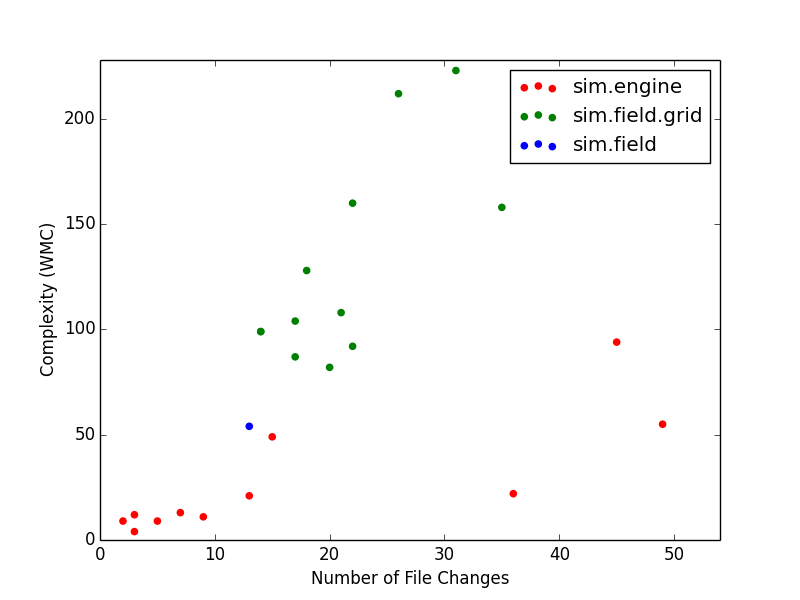
\includegraphics[width=0.8\textwidth]{Appendix/complexityVchange}
\caption{Cyclomatic Complexity and Number of File Revisions for classes in test scope}
\label{fig:complexityVchange}
\end{figure}

\begin{figure}[htp]
\centering
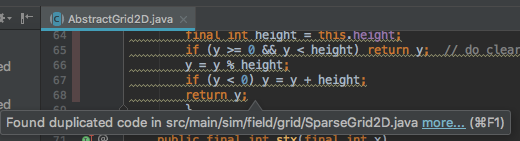
\includegraphics[width=0.8\textwidth]{Appendix/duplicated_code}
\caption{Screenshot showing IntelliJ's detection of duplicated code between AbstractGrid2D and SparseGrid2D}
\label{fig:dupe_code}
\end{figure}

\begin{figure}[htp]
\centering
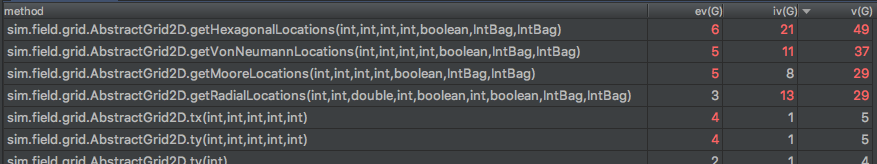
\includegraphics[width=0.8\textwidth]{Appendix/method_complexity}
\caption{\texttt{AbstractGrid2D} methods with greatest cyclomatic complexity}
\label{fig:method_complexity}
\end{figure}

\begin{figure}[htp]
\begin{subfigure}[b]{\textwidth}
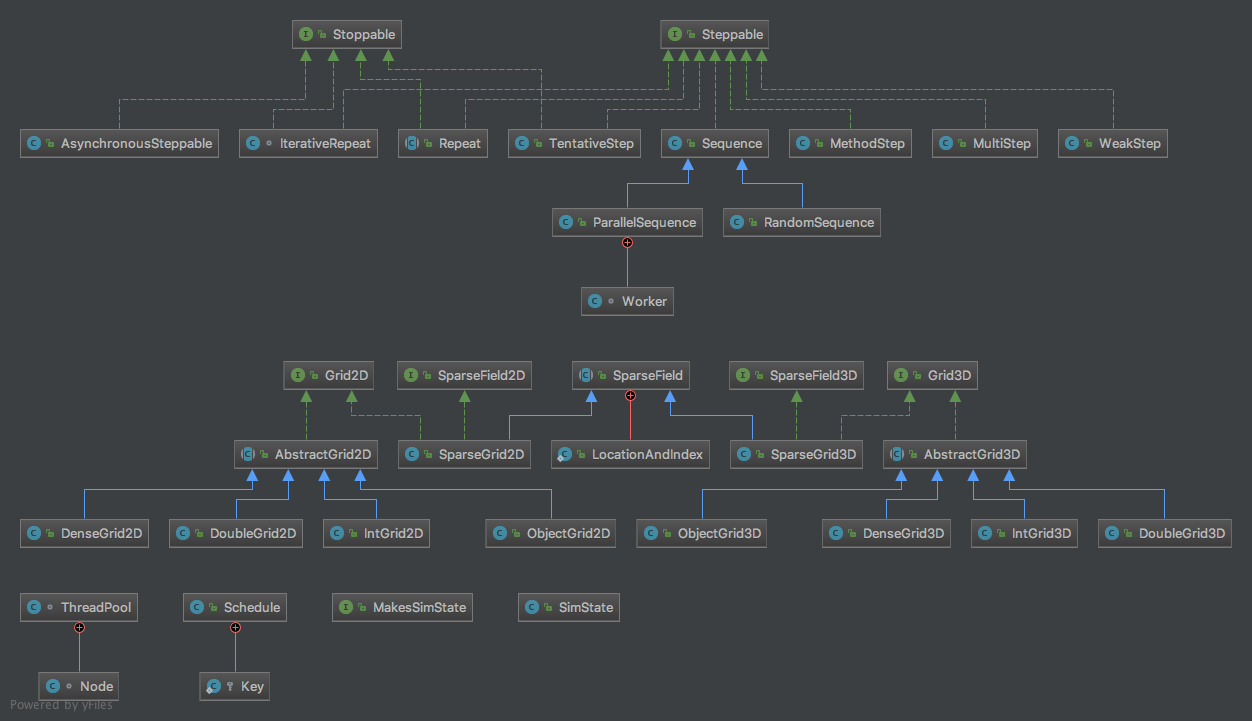
\includegraphics[width=\textwidth]{Appendix/UML}
\end{subfigure}
\begin{subfigure}[b]{\textwidth}
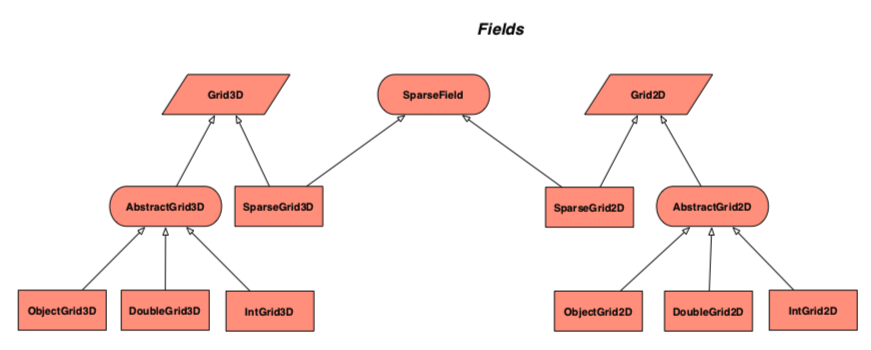
\includegraphics[width=\textwidth]{Appendix/UML_fields}
\end{subfigure}
\caption{UML diagrams of hierarchy for classes in the test scope\cite{mason_uml}}
\label{fig:uml}
\end{figure}

\begin{figure}[htp]

\begin{adjustbox}{center}
\begin{tabular}{|l|l|r|r|r|r|r|r|}
	\hline
	\multirow{3}{7.5em}{\textbf{Package}} & \multirow{3}{4em}{\textbf{Class}}
	& \multicolumn{2}{|p{3cm}|}{\textbf{HeatBugs\newline Coverage (\%)}}
	& \multicolumn{2}{|p{3cm}|}{\textbf{Tutorial 4\newline Coverage (\%)}}
	& \multicolumn{2}{|p{3cm}|}{\textbf{Mouse Traps\newline Coverage (\%)}} \\
	\cline{3-8}
	&& Method & Line & Method & Line & Method & Line \\
	\hline
	\multirow{13}{6em}{\texttt{sim.engine}}
	& AsynchronousSteppable & & & & & & \\
	& IterativeRepeat & 60 & 70 & 60 & 71 & & \\
	& MethodStep & & & & & & \\
	& MultiStep & & & & & & \\
	& ParallelSequence & 38 & 59 & & & & \\
	& RandomSequence & & & & & & \\
	& Repeat & & & & & & \\
	& Schedule & 41 & 51 & 38 & 49 & 35 & 46 \\
	& Sequence & 11 & 12 & & & &\\
	& SimState & 31 & 18 & 55 & 48 & 31 & 18 \\
	& TentativeStep & & & & & & \\
	& ThreadPool & 66 & 76 & & & & \\
	& WeakStep & & & & & & \\
	\hline
	\texttt{sim.field} & SparseField & 21 & 34 & 24 & 37 & & \\
	\hline
	\multirow{12}{6em}{\texttt{sim.field.grid}} 
	& AbstractGrid2D & 10 & 1 & 5 & 0 & 5 & 0 \\
	& AbstractGrid3D & & & & & & \\
	& DenseGrid2D & & & & & & \\
	& DenseGrid3D & & & & & & \\
	& DoubleGrid2D & 11 & 7 & 7 & 5 & & \\
	& DoubleGrid3D & & & & & & \\
	& IntGrid2D & & & & & 17 & 10 \\
	& IntGrid3D & & & & & & \\
	& ObjectGrid2D & & & & & & \\
	& ObjectGrid3D & & & & & & \\
	& SparseGrid2D & 10 & 2 & 4 & 1 & & \\
	& SparseGrid3D & & & & & & \\
	\hline
\end{tabular}
\end{adjustbox}
\caption{Code Coverage from Demo Simulation Runs}
\label{fig:coverage_heatbugs}
\end{figure}

\end{document}